\documentclass[12pt,stu,donotrepeattitle,floatsintext]{apa7}

\usepackage[american]{babel}
\usepackage{graphicx}
\usepackage{titlesec}
\usepackage{pdfpages}
\usepackage[style=apa,backend=biber]{biblatex}
\usepackage[options]{nohyperref}
\usepackage{url}
\usepackage{appendix}

\DeclareLanguageMapping{american}{american-apa}
\addbibresource{main.bib}
\linespread{2}

\newcommand{\q}[1]{``#1''}
\newcommand{\customsection}[2]{
  \phantomsection
  \section*{#1}\label{#2}
  \addcontentsline{toc}{section}{#1}
}
\newcommand{\customsubsection}[2]{
  \phantomsection
  \subsection*{#1}\label{#2}
  \addcontentsline{toc}{subsection}{#1}
}
\newcommand{\customsubsubsection}[2]{
  \phantomsection
  \subsubsection*{#1}\label{#2}
  \addcontentsline{toc}{subsubsection}{#1}
}

\title{Automated Ice Hockey Player Tracking}

\authorsnames{Douglas Code}
\authorsaffiliations{University of San Diego}
\course{AAI-521: Applied Computer Vision for AI}
\professor{Siamak Aram, Ph.D}
\duedate{December 9, 2024}

\begin{document}
    \maketitle

    \tableofcontents
    \newpage


    \customsection{Introduction}{introduction}

    The ability to track ice hockey players using computer vision presents a number of opportunities.
    Data about player positions and movements can be used for advanced statistical analysis, and team-level positioning and movements can be used to examine the strategies employed by different teams.
    For live broadcasting, player tracking allows more engaging visualizations by allowing players to be highlighted in real time for commentator discussion or graphical overlays.
    This project aimed to build a model that could take a single game video feed as input and perform five primary tasks:
    \begin{enumerate}
        \item Use object detection to locate the position of all active players in frame.
        \item Track players across frames to maintain consistent identification.
        \item Classify each player as either a skater or goalie.
        \item Classify each player as belonging to either the home team or away team.
        \item Be performant enough to be usable in real-time applications.
    \end{enumerate}

    Hockey presents a number of challenges for detection and tracking; players move quickly and occlusions are frequent and long-lasting.
    Players also largely look similar due to matching uniforms, making it more difficult to track based on appearance.
    For real-time usage, inference must also be fast enough to process 30 or 60 frames per second in order for the model to work in a live broadcast setting.

    To address these challenges, a model was developed using YOLO and ByteTrack to perform player detection, classification, and tracking.
    The resulting model shows strong performance across both all three areas, providing a capable baseline for future enhancements and visualizations.
    

    \customsection{Dataset}{dataset}

    The McGill Hockey Player Tracking Dataset (MHPTD) is a collection of 25 gameplay clips from the National Hockey League (NHL), the highest level North American hockey league.
    These clips were recorded in 30 and 60 frames per second with 1280x720 resolution by a single fixed-position camera for broadcast.
    Each clip captures a continuous sequence of gameplay with no cuts or stoppages in play.
    In all, this represents 82,305 frames with 632,785 instances of a player in the frame~\parencite{mhptd}.

    All clips are annotated using the Computer Vision Annotation Tool (CVAT) in XML format, with tracks for each unique player detailing their location in each frame.
    The annotations also include a player ID, whether they are on the home or away team, and whether they are a skater or goalie.
    The position classes (skater, goalie) are significantly imbalanced due to there typically being five skaters and one goalie on the ice at a given time for each team.
    This results in \~8.4\% of the player instances being goalies while the rest are skaters.
    Occlusions are tracked in the annotations as well, with 13.5\% of player instances being occluded in some way.

    \customsection{Preprocessing}{preprocessing}

    To get the annotations into the format expected by YOLO, the coordinates for each player-frame were parsed and normalized to a [0, 1] range relative to the frame's dimensions.
    Each instance was then encoded with one of four classes: home skater, home goalie, away skater, and away goalie.

    Clips were split into train/validation/test datasets using a 60/20/20 split.
    Splitting at the clip level allowed continuity between frames to be preserved for the tracking part of the model, and provided a better test of model efficacy by ensuring that no frames from the validation/test clips had been seen during training.
    To improve the robustness of the model, the training data frames were then augmented using a number of techniques.
    The augmentation techniques that were used are described in Table~\ref{tab:data-aug}~\parencite{yolo_train_docs}.

    \begin{table}[tb]
        \centering
        \renewcommand{\arraystretch}{0.8}
        \begin{tabular}{|l|l|}
            \hline
            \textbf{Method} & \textbf{Description}                                         \\ \hline
            Hue Adjustment        & The hue of the image is modified                       \\ \hline
            Saturation Adjustment & The saturation of the image is modified                \\ \hline
            Value Adjustment      & The brightness of the image is modified                \\ \hline
            Translation           & The image is translated horizontally or vertically     \\ \hline
            Scaling               & The image is scaled to be larger                       \\ \hline
            Flipping              & The image is flipped left-to-right                     \\ \hline
            Mosaic                & Four images are combined into a single composite image \\ \hline
            Erasing               & A portion of the image is erased                       \\ \hline
            Cropping              & Crops a portion of the image                           \\ \hline
        \end{tabular}
        \\[10pt]
        \caption{Data Augmentation Techniques}
        \label{tab:data-aug}
    \end{table}

    All images were resized to a resolution of 640x360, preserving the original aspect ratio.
    This was done to improve training and inference speed while maintaining a high enough resolution for the model to be effective.


    \customsection{Model Architecture}{architecture}

    The model is composed of a two-step pipeline: YOLO for object detection and classification and ByteTrack for object tracking.

    \customsubsection{YOLO}{yolo}

    You Only Look Once (YOLO) is an object-detection technique that performs detection in a single pass rather than using two stages, greatly improving inference speeds.
    This is done by dividing the input image into a grid and predicting bounding boxes and classifications for items centered in each grid cell.
    These bounding boxes are then combined using intersection over union (IOU) thresholds and non-max suppression to get a final predicted bounding for an object ~\parencite{yolo}.
    YOLO was chosen for this application due to its ability to handle real-time inference while maintaining high bounding-box and classification accuracy.

    \customsubsection{ByteTrack}{bytetrack}

    ByteTrack is a multi-object tracking approach that differs from competing approaches in its use of low-confidence detections.
    ByteTrack takes an initial pass to use high-confidence detections to establish motion information along with appearance similarity baselines.
    It then incorporates low-confidence detections by using the established motion and appearance information to identify which low-confidence detections are likely to be valid~\parencite{bytetrack}.
    Incorporating these detections instead of discarding them makes ByteTrack especially effective at handling occlusions compared to other techniques, which is crucial due to the frequent occlusions in ice hockey recordings.


    \customsection{Training}{training}

    During training, the nano, small, medium, and large versions of the Ultralytics YOLO v11 implementation were compared~\parencite{ultralytics_yolo}.
    The medium model offered the best balance of model complexity and performance, with the nano and small models underperforming on detection and classification for this task.
    The large model was significantly more resource-intensive to train and use than the medium model, and also was not able to achieve better predictions.
    To address the class imbalance, each class was weighted using its inverse frequency for the classification loss function.

    The trained models showed a strong tendency towards overfitting, with the training loss decreasing steadily while there was minimal improvement in validation loss even in very early epochs.
    This was addressed by introducing weight decay and dropout, as well as a 3-epoch patience interval to stop training when the performance on the validation dataset stopped improving.
    Decreasing the batch size was also found to be effective in decreasing the tendency to overfit, with a batch size of 8 being used in the final model.

    \begin{figure}[tb]
        \centering
        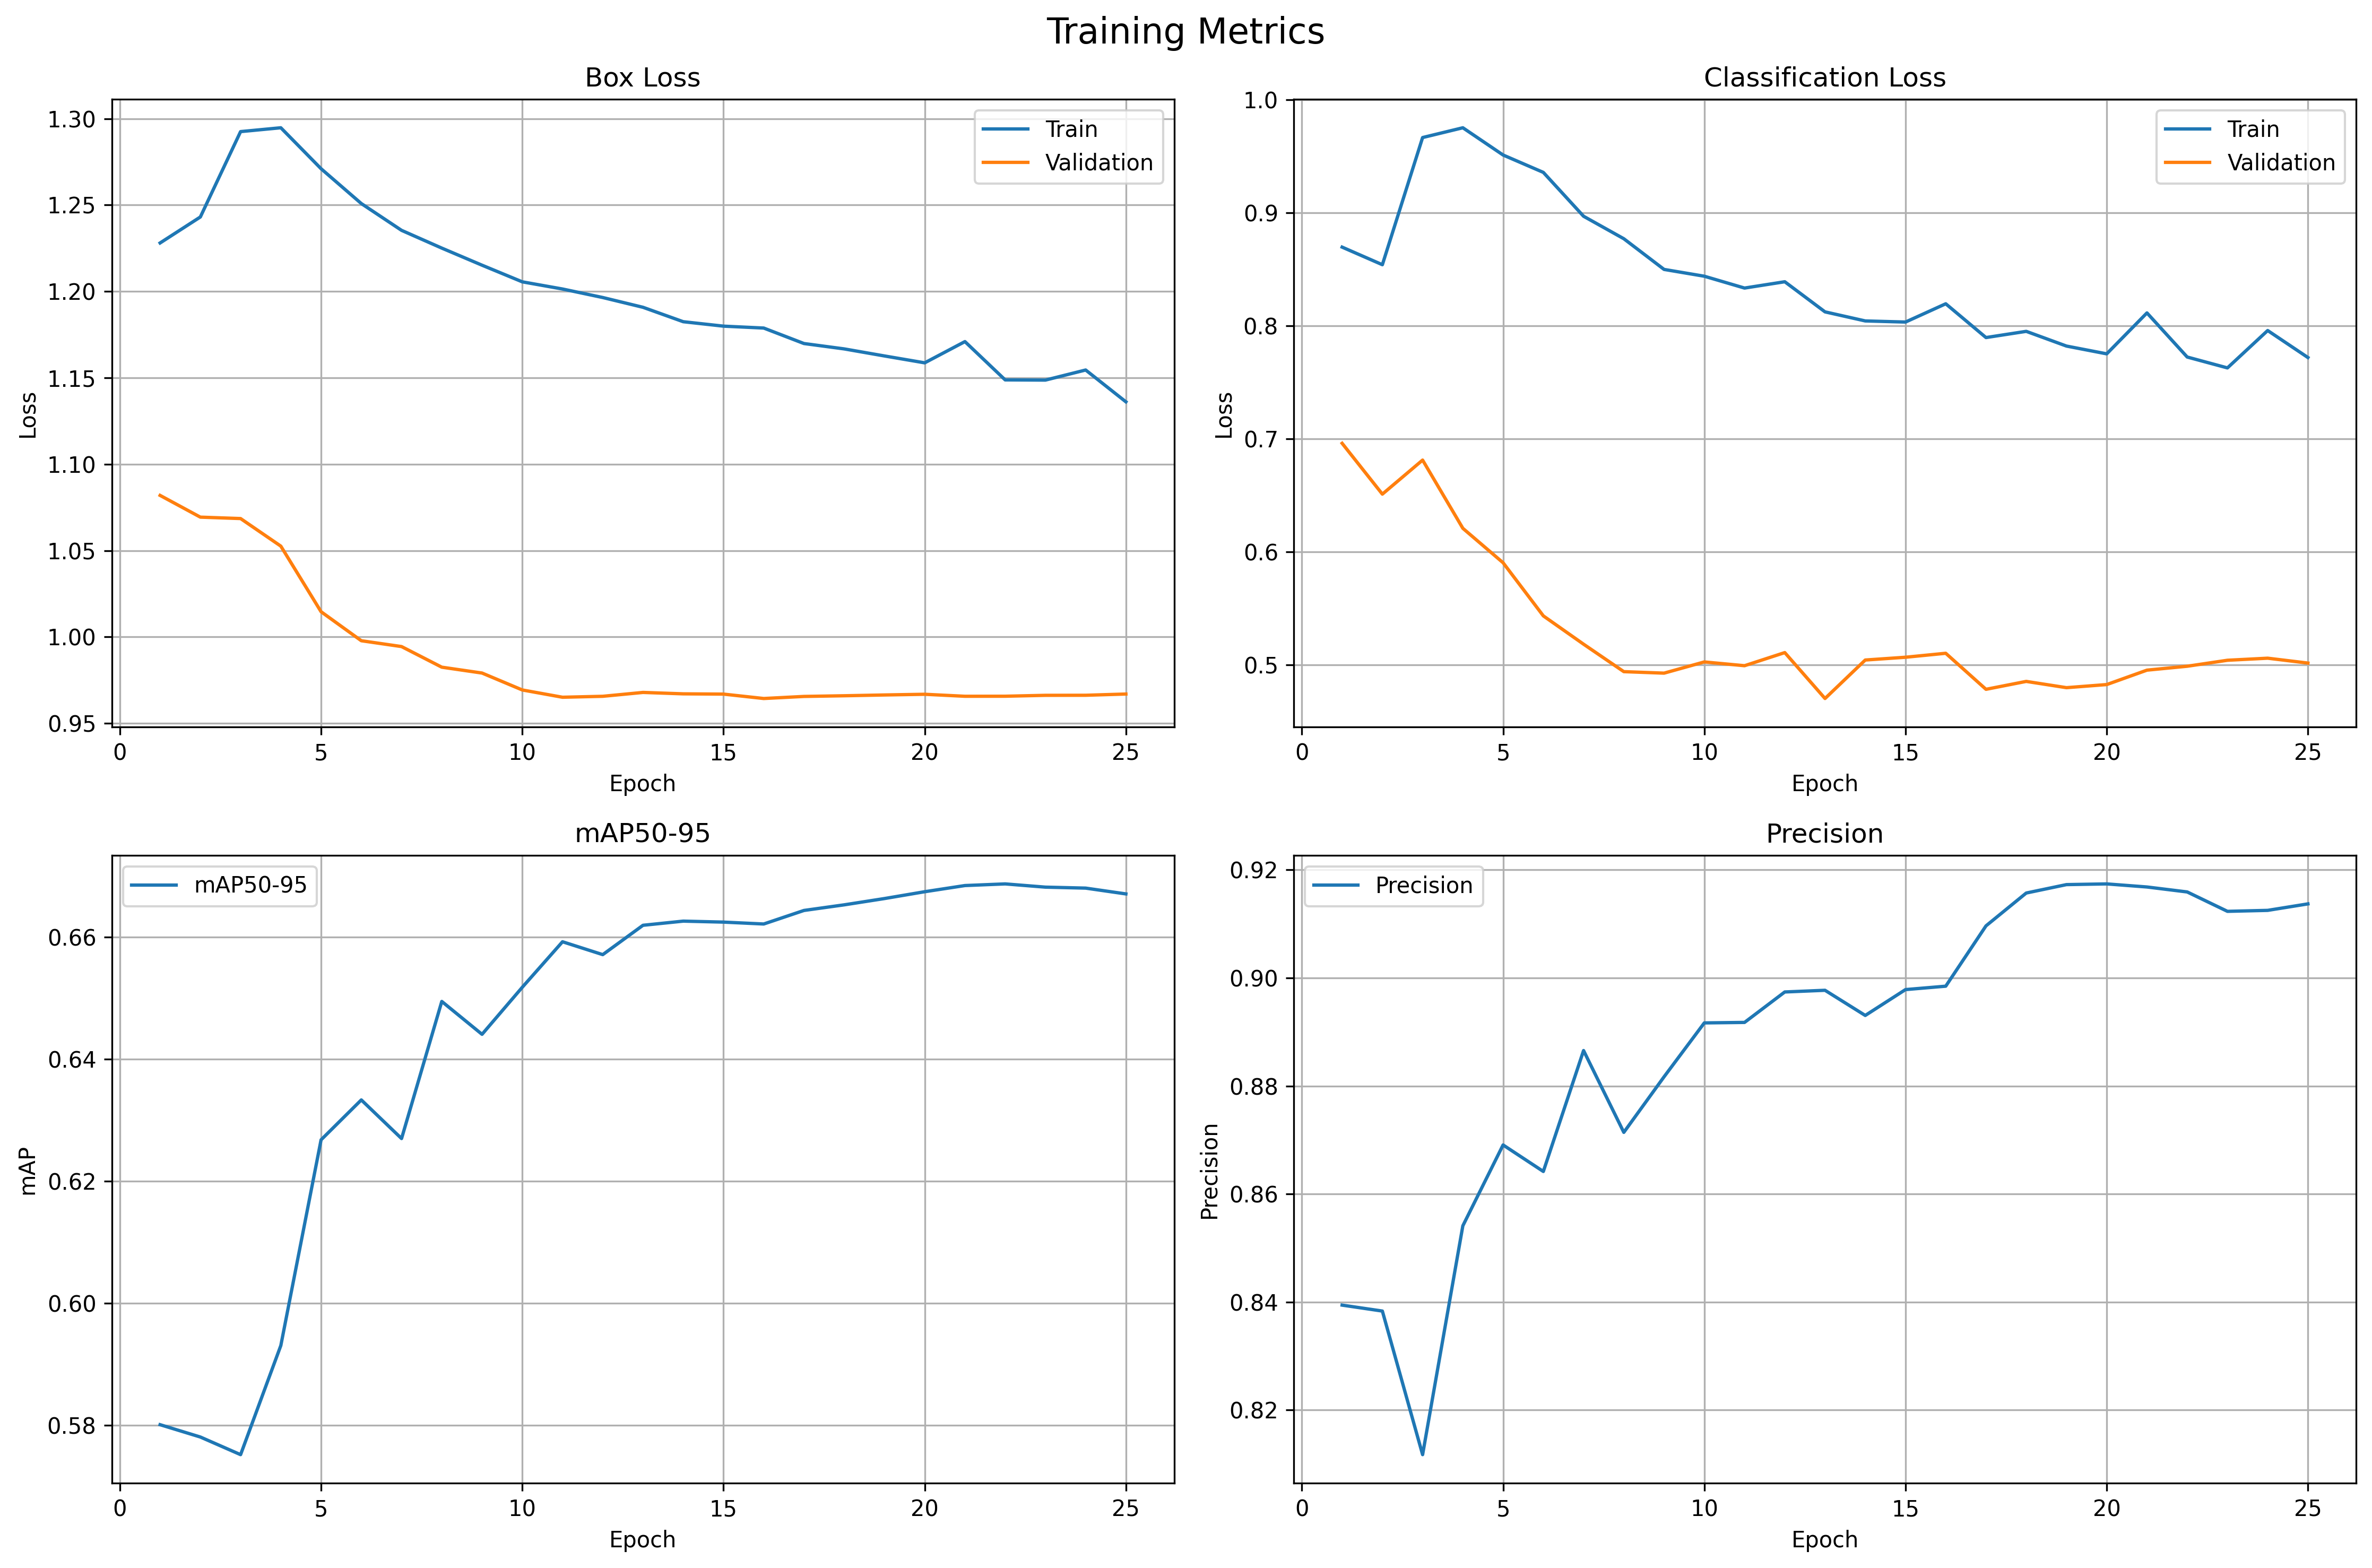
\includegraphics[width=1\textwidth]{figures/training_metrics}
        \caption{Detection model learning curves.}
        \label{fig:learning-curves}
    \end{figure}

    The learning curves, shown in Figure~\ref{fig:learning-curves}, for the final model show much less indication of overfitting, with similar improvements in both the training and validation datasets across the entire training period.
    Improvement across all metrics largely plateaus around epoch 20, and training was stopped by the early stopping mechanism at epoch 25.

    \customsubsection{Detection Model Hyperparameter Tuning}{detection-hyperparameter-tuning}

    Hyperparameter tuning for the YOLO detection model was performed using Optuna, which uses a Tree-Structured Parzen Estimator (TPE) tuner for Bayesian optimization of the hyperparameters~\parencite{optuna}.
    Using Bayesian optimization was particularly valuable for this project due to the relatively long amount of time needed for each training run.
    This allowed the tuner to converge on a high-performing set of hyperparameters much more quickly than would have been likely with a random or grid search.

    The metric used for tuning was maximization of the F1 score.
    This was chosen to balance precision (making sure detected players are actually players) and recall (making sure actual players are detected).
    The full hyperparameter ranges used and final values can be found in Appendix B.
    One notable result was the relatively high dropout value (0.7), validating the observation that overfitting was a significant issue.

    \customsubsection{Inference and ByteTrack Hyperparameter Tuning}{inference-hyperparameter-tuning}

    Key parameters for YOLO inference and ByteTrack were also tuned using Optuna.
    This tuning was done as a separate process once the final hyperparameters for the detection model fine-tuning were found.
    Running two separate hyperparameter tunings allowed the hyperparameter space to be greatly reduced for the time and resource-intensive process of fine-tuning.
    The YOLO detection confidence threshold and ByteTrack parameters were then able to be rapidly tuned using the pretrained detection model.
    The tuning metric for this secondary hyperparameter tuning was the harmonic mean of the precision, recall, multi-object tracking accuracy (MOTA), and multi-object tracking precision (MOTP):
    \[H = \frac{4}{\frac{1}{P} + \frac{1}{R} + \frac{1}{MOTA} + \frac{1}{MOTP}}\]
    The use of MOTA and MOTP is discussed further in the Evaluation section.
    Using the harmonic mean of these metrics allowed the tuning process to target a balance of precision and recall across both detection and tracking.

    The full hyperparameter ranges used and final values can be found in Appendix B.
    However, there are two notable places where the tuned ByteTrack parameters deviate significantly from the defaults: the track buffer and confidence thresholds.
    The default track buffer for determining when to remove a track is 30 frames, whereas the tuned value is 46 frames.
    This is likely due to the physical nature of hockey resulting in long occlusions as players physically battle for the puck.
    Having a higher track buffer would keep the track from being removed prematurely when players are tied up in physical engagements.
    For confidence thresholds, the default low and high track thresholds are 0.1 and 0.25, respectively.
    These are  much higher 0.46 and 0.87 in the tuned parameters.
    This could be a reflection of the strong performance of the detector, resulting in generally higher confidence values.
    Hockey has a number of features that could make detections more confident: players are constrained to a particular part of the image, wear generally consistent uniforms, and are almost always on a solid white background.
    The naturally high resulting confidence in the detection predictions could necessitate higher confidence threshholds for effective tracking as well.


    \customsection{Visualization}{visualization}
    Predictions were then visualized on each frame using bounding boxes with classification labels and track IDs.
    Each frame in a clip was then combined to create a final visualization video that had the predictions overlaid on top of the original clip.
    Figure~\ref{fig:visualization} shows a frame from one of the generated visualization clips, with each player annotated with a bounding box, their classification, and their track ID.
    The link to a full clip visualization is provided in Appendix A.

    \begin{figure}[tb]
        \centering
        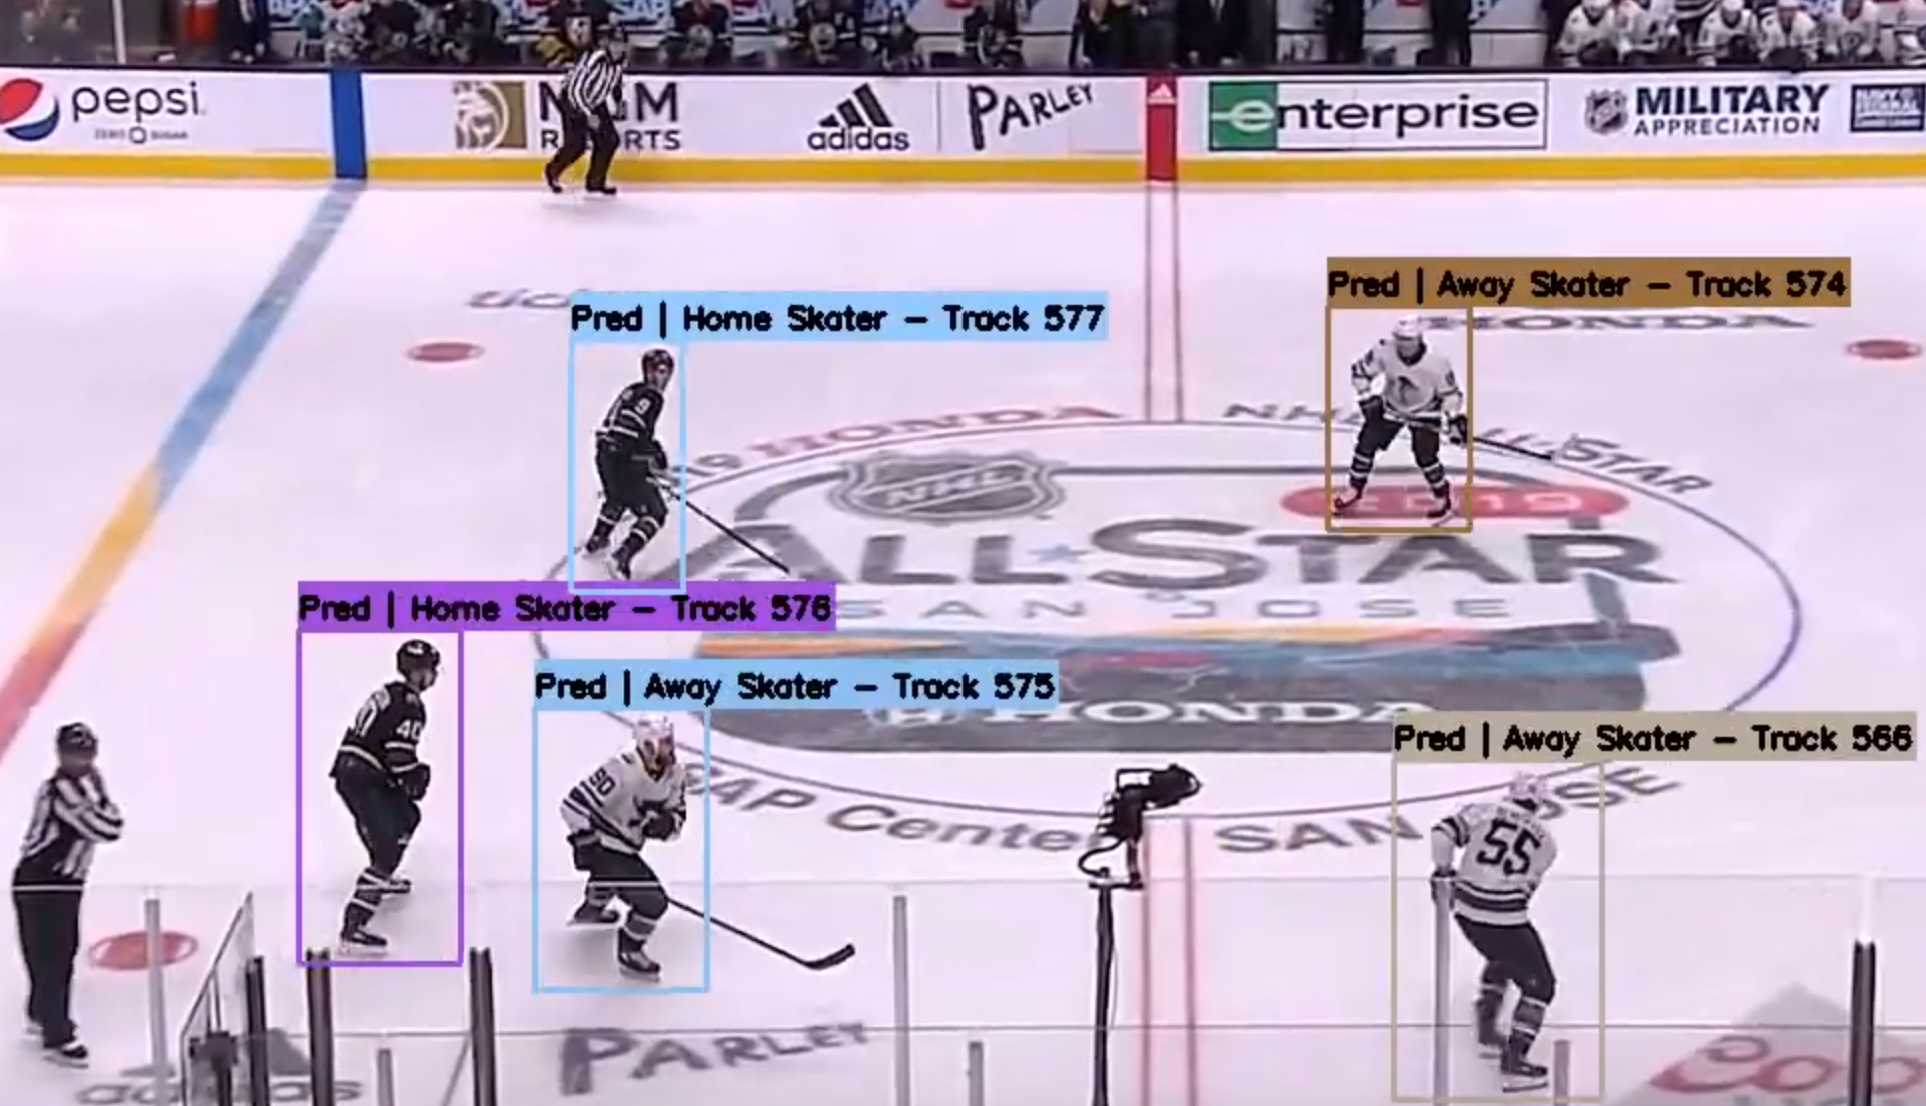
\includegraphics[width=1\textwidth]{figures/visualization}
        \caption{Example frame from visualized output clip.}
        \label{fig:visualization}
    \end{figure}

    \customsection{Evaluation}{evaluation}

    Six primary metrics were used to evaluate the model on the test dataset, as shown in Table~\ref{tab:evaluation-metrics}.

    \begin{table}[tb]
        \centering
        \renewcommand{\arraystretch}{1}
        \begin{tabular}{|p{5cm}|p{8cm}|p{2cm}|}
            \hline
            \textbf{Metric} & \textbf{Description} & \textbf{Value} \\ \hline
            Precision & The proportion of detected players that matched with actual players rather than being false detections. & 0.985 \\ \hline
            Recall & The proportion of actual players in the clip that were detected by the model. & 0.939 \\ \hline
            Multi-Object Tracking Accuracy (MOTA) & The overall tracking accuracy, accounting for missed detections, false detections, and identity switches. Ranges from -inf to 1. & 0.923 \\ \hline
            Multi-Object Tracking Precision (MOTP) & The average overlap between the predicted bounding boxes and their matching ground truth boxes. Ranges from 0 to 1. & 0.823 \\ \hline
            Track Switches & The number of times the tracker incorrectly transferred the track from one player to another. & 214 \\ \hline
            Fragmentations & The number of times a player track was incorrectly split into multiple tracks by the tracker. & 500 \\ \hline
        \end{tabular}
        \\[10pt]
        \caption{Detection and tracking evaluation metrics.}
        \label{tab:evaluation-metrics}
    \end{table}

    Overall, the model shows very strong performance in precision (0.985), recall (0.939), and MOTA (0.923), being able to correctly identify and objects and tracks quite consistently.
    The MOTP is not as high at 0.823, but still indicates a large amount of overlap with the ground truth bounding boxes.
    Examining the visualizations, the accuracy of the bounding boxes appears to be close enough that the practical implications would be minimal.

    The test dataset contains 430 tracks, meaning that the average track experiences \~1.16 fragmentations and \~0.5 track switches over the course of each clip.
    Given the frequency of players crossing paths, the relatively low number of track switches shows that the model does a fairly good job in maintaining tracks for nearby players.
    The relatively high number of fragmentations is likely due to the annotations preserving tracks for players when they're out-of-frame, whereas this model doesn't have any mechanism for identifying players themselves to preserve their tracks once the player is no longer visible.

    In terms of real-time processing for broadcast, the model was benchmarked against the test dataset and was able to process 68 frames-per-second on a mid-range consumer GPU (Nvidia RTX 3060ti).
    This suggests that the 30-60 fps needed to maintain real-time processing during a live broadcast would be easily achievable with GPU hardware appropriate for a production setting.


    \customsection{Conclusions}{conclusions}

    Using YOLO and ByteTrack, a highly effective model for ice hockey player tracking and classification was able to be created.
    The minimal computational resource requirements for the model make it viable in both analytical and real-time scenarios.

    The most valuable way to improve the model's usefulness in a production setting would be to add player identification.
    This would make the model much more valuable for both analytical and broadcast settings, as the tracking would be able to continue to follow a player even if they leave the frame and return or are occluded for long enough to lose their track.
    However, player identification is a difficult problem in this setting due to everyone of each team wearing the same uniform, as well as helmets and padding that obscure the face and body.
    One potential approach is to use jersey number recognition to identify players.
    This approach has shown some success, with researchers using the CRAFT text detection method to achieve \~87\% accuracy in detecting jersey numbers~\parencite{player-tracking}.
    Jersey number recognition does present its own issues, primarily in the fact that it requires the players' back to be visible, making it impossible to make an identification in some situations regardless of model quality.

    \printbibliography
    \clearpage

    \begin{appendices}
        \section{Appendix A: Project Links}\label{sec:project-links}
        \noindent Github repository: https://dcode15.github.io/ms-aai-520-final-project/
        \noindent Example visualization: https://www.youtube.com/watch?v=Enrnuo74tcs

        \section{Appendix B: Hyperparameter Configuration}\label{sec:hyperparameters}

        \begin{table}[tb]
        \centering
        \renewcommand{\arraystretch}{0.8}
        \begin{tabular}{|l|l|l|}
            \hline
                \textbf{Hyperparameter} & \textbf{Tuning Range} & \textbf{Final Value} \\ \hline
                Learning Rate & [0.00001, 0.01] & 0.00975 \\ \hline
                Weight Decay & [0.00001, 0.001] & 0.00024 \\ \hline
                Dropout & [0, 0.75] & 0.7 \\ \hline
                Detection Confidence Threshold & [0.1, 0.9] & \\ \hline
                IOU Threshold & [0.1, 0.9] & \\ \hline
                ByteTrack Track Buffer & [1, 120] & \\ \hline
                ByteTrack Match Threshold & [0.1, 0.9] & \\ \hline
                ByteTrack Track Low Threshold & [0.01, 0.5] & \\ \hline
                ByteTrack Track High Threshold & Low Threshold + [0.01, 0.5] & \\ \hline
                ByteTrack New Track Threshold & [0.1, 0.9] & \\ \hline
            \end{tabular}
            \\[10pt]
            \caption{Hyperparameter tuning ranges and final values.}
            \label{tab:hyperparameters}
        \end{table}

    \end{appendices}

\end{document}